\documentclass[UTF8,a4paper,11pt]{ctexart}
\usepackage[margin=2.2cm]{geometry}
\usepackage{amsmath,amssymb,amsthm,bm,booktabs,longtable,array,graphicx,xcolor}
\usepackage{enumitem,hyperref,fancyhdr,placeins}
\hypersetup{colorlinks=true,linkcolor=blue!50!black,urlcolor=blue!50!black,citecolor=blue!50!black}
\setlist{nosep,leftmargin=2em}
\setlength{\headheight}{15pt}
\pagestyle{fancy}\fancyhf{}\fancyhead[L]{连续随机DR与冻结候选验证}\fancyhead[R]{实现与实测说明}\fancyfoot[C]{\thepage}
\newcommand{\E}{\mathbb E}\newcommand{\Prb}{\mathbb P}\newcommand{\R}{\mathbb R}
\newcommand{\Tcal}{\mathcal T}\newcommand{\ind}{\mathbf 1}
\newtheorem{proposition}{命题}
\newtheorem{remark}{说明}
\title{连续随机需求响应与RNJ＋WZZT冻结候选验证\\\large 完整模型、条件积分、局部求解与AC测试}
\author{研究实现说明：异质资源概率可行化版本}
\date{版本：probability-refinement-v1}
\begin{document}\maketitle
\begin{abstract}
本文描述一个已经接入代码的24小时连续需求响应（DR）问题：从完整历史观测构造RNJ＋WZZT候选，冻结其结构、响应矩阵和输出映射；以最小服务费选择节点、资源、时段和幅度，使当前候选退出原3\%验证带的规划概率达到95\%。资源包括用户移位、用户削减、单向EV充电和家庭储能。响应包含节点相关、时间相关和整日偏差，实际交付经功率、能量、到离站和SOC约束控制。绝对值残差的符号随决策和随机量变化，采用一维高斯条件积分计算事件概率；外层使用固定随机积分点，求解器使用其梯度。新增改进仅处理概率平坦区的初值及可行化、费用下降和独立核验，不改变候选、负荷、噪声、设备库存或3\%规则。95\%属于声明工作分布下的激励事件；实际效果由另取整日路径、原交流潮流和表计噪声后的最终错漏评价。
\end{abstract}
\tableofcontents\newpage

\section{任务、信息边界与当前算法}
\subsection{要优化的对象}
一个新日有96个15分钟时段。优化器在新日开始前读取历史P/Q/V、冻结的预测模型和可调设备，不读取新日实际负荷、响应或真实拓扑。优化之后冻结整个合同，再模拟或执行新日，最后按原验证和输出规则选模。

当前实现的辨识作用发生在\textbf{冻结候选的验证回选}。历史RNJ＋WZZT已提供完整族、各族共同拟合的R/X及后处理输出；本次价格搜索和新日评分不重新估计线路参数，也不重新运行WZZT结构搜索。因而，得到正确历史候选属于联合流程的作用，不能写成新日发现了候选池外的线路。

\subsection{保留和改变了什么}
保留三个已声明条件、每例288行训练和288行验证、历史候选及全部参数、新日权重2、统一3\%验证带、原0.16输出映射、设备库存、噪声和响应规律。没有货币预算上限；最小费用受物理资源能力限制。所有节点均可参与，不强制分散、不固定节点编号。

本轮在旧算法上增加：未达标尾部初值、较完整但有上限的局部搜索、128个外层规划积分点、4096个独立概率核验点，以及严格的“规划可行／仅诊断”输出分类。尾部指标仅辅助数值搜索，最终仍检查原损失差事件。

\section{符号、维度与单位}
\begin{longtable}{p{.18\textwidth}p{.74\textwidth}}
\toprule 符号&含义及单位\\\midrule\endhead
$n,T,\Delta t$&终端节点数，$T=96$，$\Delta t=0.25$小时。\\
$i,t,j$&节点、15分钟时段、资源编号；每节点有4类资源，$j=1,\ldots,4n$。\\
$i(j),\kappa_j$&资源所属节点、资源无功增量/有功增量比例。用户取0.2/0.35/0.5，EV与储能取0。\\
$p_t,q_t,y_t$&节点有功、无功（标幺）；$y_{it}=v_{0t}^2-v_{it}^2$（标幺平方）。\\
$R_k,X_k$&冻结候选$k$的$n\times n$响应矩阵。它们是$y=Rp+Xq$中的系数，不直接等于原始欧姆阻抗。\\
$C,F$&当前历史选中候选、一个历史相容的竞争候选；名称不代表谁是真实拓扑。\\
$R_0,X_0$&历史拟合的非树参考预测矩阵；用于规划生成参考电压，不是已知真值。\\
$H_k,L_k,S_k$&历史验证平均绝对误差、新日平均绝对误差、加权合并验证误差。\\
$D,h$&新日损失差$L_C-1.03L_F$及其排除阈值；均为标幺平方。\\
$A_{jt}^+,A_{jt}^-$&相对原设备基线的增负荷/减负荷裕量（kW），均非负。\\
$x_{j\ell},u_{jt},U_{jt}$&24个小时控制坐标、名义资源调节（kW）、随机实际交付（kW）。\\
$c_{jt},\pi_{jt},\mathcal C(u)$&满激活服务单价、实际合同单价（元/kWh场景假设）、固定预付服务费（元）。\\
$Z,\nu,m$&标准化相关行为误差、相对标准差、平均履约倍率。\\
$z,\zeta,\eta$&标准高斯背景因子；一维被积分因子；与之独立的其余因子。\\
$\Tcal$&因果设备控制器：饱和并保持能量任务可完成。\\
$N,M$&外层积分点数、每个新日候选的残差单元数$M=nT$。\\
\bottomrule
\end{longtable}
全文公式使用标幺平方误差。实现为改善数值尺度，将残差、$D$和$h$统一乘$10^6$；图表称为“微标幺平方”。概率和选择规则在共同正缩放下不变。功率调节由kW除以该例的\texttt{base\_kw}后才能进入R/X。

\section{历史辨识与可复用的验证排除条件}
\subsection{候选与参数固定}
WZZT使用共同层状块结构，单个候选族$\mathcal F_k$的响应为
\begin{equation}
 R_k=\sum_{B\in\mathcal F_k}r_{kB}z_Bz_B^\top,
 \qquad X_k=\sum_{B\in\mathcal F_k}x_{kB}z_Bz_B^\top,
 \quad r_{kB},x_{kB}\geq0.
\end{equation}
$z_B$是块$B$的节点指示向量。历史拟合允许同族全部权重共同变化，包含零和弱权重。现有候选来自完整RNJ树库和WZZT历史路径；此次比较从历史最终输出确有差异的候选中固定$C,F$，保持各自\emph{完整}联合族及其R/X，而非只保留争议块。优先使用历史下一接受路径点，否则按已声明的历史竞争规则选取。没有历史最终争议时保留零采购对照。

冻结之后，对任意新日观测，候选预测和损失为
\begin{equation}
 \widehat y_{kt}=R_kp_t^m+X_kq_t^m,
 \qquad L_k=\frac1{nT}\sum_{t=1}^{T}\sum_{i=1}^{n}|y_{it}^m-\widehat y_{kit}|.
 \label{eq:loss}
\end{equation}
这里上标$m$表示实际表计数据。不再为每个新日或DR动作重调$R_k,X_k$。

\subsection{3\%带到激励阈值的等价推导}
历史验证288行，新日96行且权重2。因此
\begin{equation}
 S_k=\frac{288H_k+2\times96L_k}{480}=0.6H_k+0.4L_k.
\end{equation}
历史筛选先保留$H_k\leq1.03\min_jH_j+\varepsilon$的候选。对保留的两个候选，若$C$满足
\begin{equation}
 S_C>1.03S_F+\varepsilon,\qquad\varepsilon=10^{-12},
\end{equation}
则$F$一定是二者中损失较小者，$C$退出3\%带。移项得到
\begin{equation}
 \boxed{D:=L_C-1.03L_F>h:=1.5(1.03H_F-H_C)+2.5\varepsilon.}\label{eq:threshold}
\end{equation}
阈值只由冻结历史、样本权重和原规则决定，不另加120\%目标或自造裕量。严格不等式与实际候选带的闭区间规则对应。边界相等时不排除。

若候选池超过两个，$C$退出相对$F$的带是排除$C$的充分条件，最终哪个候选被选仍取决于整个池。本次数值只有两个完整候选，报告这一范围。

实际选择在验证带中按原始支撑数、损失、冻结顺序比较，之后采用冻结的0.16输出映射。$D>h$表示排除当前候选，并不预设这次排除一定正确；必须在选后用真实网络核算错漏。零收益对照也用同一规则。

\section{资源库存、报价与服务费}
\subsection{历史负荷到可调库存}
节点尺度$s_i$取训练正净负荷的90\%分位数，网络总可调库存设为$0.20\sum_i s_i$。节点库存乘预锁的0.8/1/1.2尺度后归一化；用户、EV、储能按三种预锁组成分配，分别为65/20/15、30/50/20和35/20/45（\%）。用户部分再分75\%移位、25\%削减。分配只看训练有功与节点标号的固定散列，不看测试错误或真实分支。未声明电网终端调节设备，因此该类分配为零。

当前三例库存为21.5964、19.4048、22.9033 kW。它们是合成可签约资产，不由净负荷自动推断为真实设备。这一全库存域与早期2 kW域不同；本轮对照均使用相同全库存。

\subsection{连续报价的可逆表示}
正$u$为增加用电，负$u$为减少用电。给定方向的功率裕量$A_{jt}^{\operatorname{sgn}u}$，简化响应曲线为
\begin{equation}
 |u_{jt}|=A_{jt}^{\operatorname{sgn}u}\frac{\pi_{jt}}{c_{jt}},\quad
 0\leq\pi_{jt}\leq c_{jt},\quad
 \pi_{jt}=c_{jt}\frac{|u_{jt}|}{A_{jt}^{\operatorname{sgn}u}}.
\end{equation}
无方向裕量时强制$u_{jt}=0$。这里的$u$是合同名义调节，并非控制饱和后的无条件均值。报价代表服务补偿，未加入零售电价或重复计算储能磨损。

预付服务费为
\begin{equation}
 \boxed{\mathcal C(u)=\Delta t\sum_{j,t}c_{jt}\left(\frac{(u_{jt}^{+})^2}{A_{jt}^{+}}+
 \frac{(u_{jt}^{-})^2}{A_{jt}^{-}}\right),\quad
 u^+=\max(u,0),\quad u^-=\max(-u,0).}\label{eq:cost}
\end{equation}
同设备同槽不会同时选择两种方向。各资源分别计费后才在节点上相加，不能利用相反调节净额抵消费用。费用在冻结合同后确定，未履约不重抽随机数、不重新报价；实际调节量、控制器补偿量和实际磨损费用代理另列。

\begin{table}[ht]\centering\small
\caption{基础满激活补偿单价（元/kWh，合成场景参数）}
\begin{tabular}{lccccc}\toprule
资源&00--06&06--09&09--17&17--22&22--24\\\midrule
用户&0.60&1.00&0.80&1.20&0.70\\
EV&0.30&0.60&不可用&0.45（18时后）&0.30\\
储能&0.30&0.35&0.30&0.50&0.35\\\bottomrule
\end{tabular}\end{table}
另乘节点0.9/1/1.1费用因子。成本量级、弹性斜率、库存比例和行为标准差均属明确假设，不能称实证校准；旧实验的合同单位也不据此换算成人民币。

\section{设备可行域与因果执行}
\subsection{移位、削减、EV与储能}
用户移位设备基线$b_{jt}=a_jv_t$，$v_t$依五时段取0.6/1/0.8/1/0.7；增量$u\in[-b,b]$，累计移位能量在$[-2a_j,2a_j]$ kWh内，日终为零。削减设备$u\in[-b,0]$，全日削减不超过$2a_j$ kWh，无偿还要求。

EV以7 kW、50 kWh、每夜20 kWh电网侧补能为等比合同份额。连接时段00--08和18--24，基线在14小时内恒定充电；可削减裕量约为铭牌20.41\%，可增加约79.59\%。无V2G，效率0.9，SOC20\%--90\%，18时到站SOC40\%。前夜在00时前已完成6/14任务；00--08完成余下8/14。新晚18--24完成6/14。\emph{两个连接段分别令增量能量为零}，防止跨离站时间借用充电量。单向充电与这些固定服务量保证该模板SOC范围，核验仍重新计算SOC。

储能功率$a_j$，容量$2.5a_j$ kWh，SOC20\%--80\%、初末50\%；充放效率均为$\eta_b=\sqrt{0.85}$。
\begin{equation}
 e_{j,t+1}=e_{jt}+\Delta t\left(\eta_bU_{jt}^{+}-\frac{U_{jt}^{-}}{\eta_b}\right),
 \quad -0.75a_j\leq e_{jt}\leq0.75a_j,\quad e_{j,0}=e_{j,T}=0.
\end{equation}
其净购电可以为正以补偿损耗，不能将绝对调节量等同净新增用电。用户无功响应按节点$\kappa_j$变化，EV与储能无功增量为零。

\subsection{控制器的精确定义}
仅逐槽截断会破坏日终能量和EV离站服务。现有控制器$\Tcal$根据当前状态和未来已知能力保留可完成性。设$f_j(p)=\eta_jp$（$p\geq0$）、$p/\eta_j$（$p<0$），用户及EV的增量电网能量取$\eta_j=1$。给定到当前服务段终点的未来最低/最高能量$F^-_{jt},F^+_{jt}$，先确定
\begin{align}
 \underline e^{\rm next}_{jt}&=\max(\underline e_j,-F^+_{jt}),&
 \overline e^{\rm next}_{jt}&=\min(\overline e_j,-F^-_{jt}),\\
 \ell_{jt}(e)&=\max\left(-A^-_{jt},f_j^{-1}\left(\frac{\underline e^{\rm next}_{jt}-e}{\Delta t}\right)\right),\\
 r_{jt}(e)&=\min\left(A^+_{jt},f_j^{-1}\left(\frac{\overline e^{\rm next}_{jt}-e}{\Delta t}\right)\right).
\end{align}
再执行
\begin{equation}
 U_{jt}=\operatorname{clip}(V_{jt},\ell_{jt}(e_{jt}),r_{jt}(e_{jt})),\qquad
 e_{j,t+1}=e_{jt}+\Delta t f_j(U_{jt}).\label{eq:controller}
\end{equation}
削减资源不加日终偿还区间。EV各连接段重置增量状态。控制器不读取未来随机响应；它只读取未来已声明的功率上限和截止时间。

\begin{proposition}[设备可完成性]
在本模板的确定可用性、连续功率区间、初始可行状态及准确设备执行下，式\eqref{eq:controller}产生的每段状态都保持在可完成区间内，最终达到规定增量能量；同时满足功率和累计能量界。
\end{proposition}
理由是当前功率界与可完成下一状态的逆像取交，下一状态仍存在满足未来能力的延续；递推至最后一槽时未来能量为零，区间收缩到目标。此保证针对设备模型，不覆盖突然离站、设备故障或电网热限。控制器存在意味着采用带本地自动控制的服务合同；仅给任意居民发送价格且完全自愿执行，不能自动获得同样的终端保证。

\section{连续随机响应及其协方差}
\subsection{价格到意向响应}
冻结$u$后，未受设备控制的意向增量为
\begin{equation}
 V_{jt}=u_{jt}(m+\nu_{jt}Z_{jt}),\qquad
 U=\Tcal(V).\label{eq:response}
\end{equation}
主模型$m=1$；用户、EV、储能基础$\nu$为0.15、0.08、0.03，另乘节点误差因子0.9/1/1.1。用户06--09及17--22再乘1.25，EV06--08再乘1.5。价格提高同时增加意向均值和绝对标准差，避免把买到的更大响应当作无误差控制。

\subsection{整段相关结构}
令$g$为共同日因素、$g_i$为节点日因素、$a_t$为共同AR(1)因素、$b_{jt}$为资源AR(1)因素；四类标准高斯源相互独立，AR过程以标准正态平稳初始化。取
\begin{align}
 Z_{jt}&=\sqrt{\omega_0}g+\sqrt{\omega_1}g_{i(j)}+\sqrt{\omega_2}a_t+\sqrt{\omega_3}b_{jt},\\
 a_t&=\phi a_{t-1}+\sqrt{1-\phi^2}\epsilon_t,
 \qquad\sum_{r=0}^{3}\omega_r=1.
\end{align}
于是
\begin{equation}
 K_{jt,ks}=\omega_0+\omega_1\ind_{i(j)=i(k)}+
 (\omega_2+\omega_3\ind_{j=k})\phi^{|t-s|},\label{eq:cov}
\end{equation}
\begin{equation}
 \E V_{jt}=mu_{jt},\quad
 \operatorname{Cov}(V_{jt},V_{ks})=u_{jt}u_{ks}\nu_{jt}\nu_{ks}K_{jt,ks}.
\end{equation}
因子构造保证协方差半正定；异号动作可以产生负的增量协方差。主参数为
\begin{equation*}(\omega_0,\omega_1,\omega_2,\omega_3)=(.15,.25,.20,.40),\qquad\phi=.8.\end{equation*}
失配核验使用$m=.9$、方差份额$(.30,.30,.25,.15)$及$\phi=.9$，不重新优化报价。

$U=\Tcal(V)$通常有边界点质量，既非高斯，也不满足$\E U=u$。因此本算法没有直接套用$\mu-1.645\sigma\geq h$；它将控制后的完整响应纳入积分。报价与方差、相关性均进入优化，而非只优化均值后补噪声。

\section{背景预测与参考电压}
\subsection{现用工作分布}
每例使用三个完整训练日。将同槽背景P/Q及非树参考预测残差连接为向量
\begin{equation}
 W^{(d)}=\operatorname{vec}\left(P^{(d)},Q^{(d)},
 Y^{(d)}-P^{(d)}R_0^\top-Q^{(d)}X_0^\top\right),\quad d=1,2,3.
\end{equation}
以同槽均值为预测，使用
\begin{equation}
 W=\bar W+B_Wz,\quad z\sim N(0,I_3),\qquad
 B_W=\frac1{\sqrt2}[W^{(1)}-\bar W,W^{(2)}-\bar W,W^{(3)}-\bar W].
\end{equation}
背景与行为因子$Z$暂设独立。该协方差秩最多2，是当前计算的工作假设，不是充分校准的未来误差分布。资源库中另有分时5/10/8/10/5\%背景误差模板，但\textbf{本批未接入}，不能将其写成已实现随机量。

\subsection{DR如何改变候选残差}
资源增量聚合为
\begin{equation}
 \Delta p_{it}=\frac1{P_{\rm base}}\sum_{j:i(j)=i}U_{jt},\qquad
 \Delta q_{it}=\frac1{P_{\rm base}}\sum_{j:i(j)=i}\kappa_jU_{jt}.
\end{equation}
参考模型按$R_0\Delta p+X_0\Delta q$传导DR。候选$k$的新日残差向量可直接写成
\begin{equation}
 r_k=\mu_k+B_kz+G_k\operatorname{vec}U,\label{eq:residual}
\end{equation}
其中$\mu_k,B_k$由三个训练日的候选残差均值和中心化列构成。$G_k$按时段分块，每个资源对应列为
\begin{equation}
 g_{kj}=\frac{(R_0-R_k)_{:,i(j)}+\kappa_j(X_0-X_k)_{:,i(j)}}{P_{\rm base}}.
\end{equation}
这使位置、资源P/Q特性、方向和幅度直接影响\emph{同一验证损失}。两个候选R/X的预测差大，不必然意味着相对实际电压的误差差大；式\eqref{eq:residual}仍依赖参考电压模型。实际AC检验正是检查这一依赖是否有效。

规划中历史联合残差包含历史噪声的部分影响，但未单独追加满秩新日电压与P/Q表计误差。实际核算另加原噪声。因此规划概率与AC达成率可有系统差异，此限制不能仅靠增加积分样本消除。

\section{完整概率优化问题}
为减少时间变量而不固定节点，令$x_{j\ell}$为24小时控制坐标，$\ell=1,\ldots,24$，每小时展开4个槽。定义$s_{jt}=\max(A_{jt}^+,A_{jt}^-)$，
\begin{equation}
 v_{jt}(x)=s_{jt}x_{j,\lceil t/4\rceil},\qquad
 u(x)=\Tcal(v(x)),\qquad U(x,Z)=\Tcal(u(x)\odot(m+\nu\odot Z)).
\end{equation}
名义控制器可能为完成服务在小时内调整各槽；因此$x$是小时请求坐标，最终价格由每槽$u$反算。两次控制分别保证名义合同与随机交付可行。

完整问题为
\begin{equation}
\boxed{\begin{aligned}
 \min_x\quad &\mathcal C(u(x))\\
 \text{s.t.}\quad
 &\Prb_{z,Z}\left\{\frac{\|r_C(x,z,Z)\|_1-1.03\|r_F(x,z,Z)\|_1}{M}>h\right\}\geq0.95,\\
 &-1\leq x_{j\ell}\leq1 &&\text{移位、EV、储能},\\
 &-1\leq x_{j\ell}\leq0 &&\text{削减},\\
 &u=\Tcal(v(x)),\quad U=\Tcal(u\odot(m+\nu\odot Z)),\\
 &\pi_{jt}=c_{jt}|u_{jt}|/A_{jt}^{\operatorname{sgn}u},\quad 0\leq\pi_{jt}\leq c_{jt}.
\end{aligned}}\label{eq:program}
\end{equation}
设备功率、能量与SOC约束通过$\Tcal$逐路径满足。电网电压/热限不在本批优化约束内，电压在AC执行后核验；热限未核。所有随机性只作用于当前定义的背景与连续行为，不包括未知拓扑的随机先验。

该问题是分段可微的非凸概率约束问题，\textbf{不是当前已经精确化为SOCP或MILP的问题}。若符号和控制分区均固定且损失差恰为高斯仿射函数，才可局部使用高斯分位数形式；本实现不依赖这种固定符号近似。

\section{不固定正负号的条件积分}
\subsection{对谁积分}
取历史固定单位方向$d\in\R^3$及正交补矩阵$N_d$，将背景因子写成
\begin{equation}
 z=d\zeta+N_d\eta,\qquad \zeta\sim N(0,1),\quad\eta\sim N(0,I_2),\quad\zeta\perp\eta.
\end{equation}
代码以历史均值残差符号给出的背景敏感方向选$d$，零方向时使用领先奇异向量。这只选择积分轴，不将该符号作为以后损失的固定符号。

固定外层$(\eta,Z)$后，设备交付$U(x,Z)$已确定，各候选残差沿$\zeta$为仿射函数。将两候选连接为
\begin{equation}
 D(x,\zeta;\eta,Z)=\sum_{a=1}^{2M}w_a|\gamma_a(x;\eta,Z)+\beta_a\zeta|,
 \quad w=\frac1M(\ind_M,-1.03\ind_M).
\end{equation}
$\gamma$中的$U$随$x$变化；$\beta=(B_Cd,B_Fd)$在当前模型中固定。

\subsection{精确的一维概率}
排序所有非零$\beta_a$对应的折点$-\gamma_a/\beta_a$。每两个折点之间，所有残差符号确定，$D$是一条直线；解$D>h$得到若干区间$(l_r,u_r)$。因此
\begin{equation}
 p(x\mid\eta,Z)=\sum_r[\Phi(u_r)-\Phi(l_r)].\label{eq:integration}
\end{equation}
这是给定外层因素的一维高斯积分，而非用均值代替随机性。区间可以不连续，正负权重均保留，零斜率和零残差单独处理。复杂度为每外层点$O(M\log M)$。

总概率仍为$\E_{\eta,Z}p(x\mid\eta,Z)$。实际用预锁的独立外层点计算
\begin{equation}
 \widehat p_N(x)=\frac1N\sum_{s=1}^N p(x\mid\eta_s,Z_s),\qquad N=128.
\end{equation}
外层随机积分是计算连续分布的数值方法，并非把现实响应改成只有128个可能状态。对一个冻结报价另用4096个独立点核验，不将核验点回流选价。

\section{梯度来自哪里}
\subsection{概率边界的导数}
设条件事件的边界根$\rho$满足$D(x,\rho)=h$，不位于残差折点且$D_\zeta(x,\rho)\ne0$。隐函数求导与区间高斯质量求导给出
\begin{equation}
 \nabla_x p(x\mid\eta,Z)=\sum_{\rho:D(x,\rho)=h}
 \frac{\phi(\rho)}{|D_\zeta(x,\rho)|}\nabla_xD(x,\rho).\label{eq:gradient}
\end{equation}
根处的残差符号来自当前$x$与当前根，而非历史平均符号。程序通过排序根及前缀和构造$\gamma$系数梯度，再乘$G_C,G_F$，反向通过实际控制器、随机倍率、名义控制器和小时展开映射。

固定控制分区时，$U_t$对当前请求及状态的局部导数分别为$\mathsf A_t,\mathsf B_t$，状态对功率的导数为$\mathsf K_t=\Delta tf'(U_t)$。对反向状态伴随量$\lambda_{t+1}$，链式法则为
\begin{equation}
 \psi_t=g_t+\mathsf K_t\lambda_{t+1},\quad
 \frac{\partial J}{\partial V_t}=\mathsf A_t\psi_t,\quad
 \lambda_t=\lambda_{t+1}+\mathsf B_t\psi_t.
\end{equation}
服务段起点重置伴随状态。控制切换点采用当前面导数并以真实函数值线搜索；因此局部方法不保证全局最优。

\subsection{导数有效性与积分误差}
条件概率在阈值平台、阈值落在绝对值折点或活动零残差处可能不可微，代码显式标记导数未决，不将零数组冒充可靠梯度。对有限个已锁外层点，在各点局部可微时可以直接求和得到$\nabla\widehat p_N$。若要进一步声称等于连续外层真概率的无偏梯度，还需可积支配等条件；本报告不作该保证。

独立核验返回平均值、标准误和一个有明确条件的界。对冻结决策及$i.i.d.$的$X_s=p(x\mid\eta_s,Z_s)\in[0,1]$，Hoeffding不等式给出
\begin{equation}
 p(x)\geq\bar X-\sqrt{\frac{\log20}{2N_q}},\qquad N_q=4096,
\end{equation}
其概率至少为95\%，只针对\emph{所声明工作分布的数值积分误差}。该下界不用于重新选择报价，不证明工作分布符合实际电网。规划95\%、独立估计值、该下界和AC达成率分别报告。

\section{本轮求解改进：尾部初值、原概率约束与降费}
\subsection{为什么只做概率梯度可能停住}
若当前所有条件边界远在高斯尾部，$\phi(\rho)$很小，概率梯度可能近零。此时“小请求到不了阈值”不等于整个物理域无解。旧实现每阶段20步、32外层点且仅用均值初值，三个条件均未找到95\%可行报价。

本轮保留旧报价作为开发初值；先优化同一$D$的期望，再针对$h-D$的上尾作初值改进，之后回到原概率。上尾使用标准的条件风险表达\cite{rockafellar}：
\begin{equation}
 \min_{x,\alpha}\left\{\alpha+\frac1{0.05}\E[(h-D(x)-\alpha)_+]\right\}.\label{eq:tail}
\end{equation}
它可推动那些仍低于阈值的路径，避免只推高已有成功路径。本式仅用于初始化，既不替代\eqref{eq:program}，也不因其值为正便宣称原概率问题无解。控制和有符号绝对值差仍使其关于$x$非凸。

\subsection{尾部也能精确条件积分}
固定外层后令$\tau=h-\alpha$、$I=\{\zeta:D(\zeta)<\tau\}$。先用原区间算法求$I$，再求
\begin{equation}
 J(\tau)=\E[(\tau-D)_+]=\tau\Prb(I)-\sum_a w_a\E[|\gamma_a+\beta_a\zeta|\ind_I].
\end{equation}
每个区间的质量为$\Phi(u)-\Phi(l)$，一阶矩为$\phi(l)-\phi(u)$；再在$-\gamma_a/\beta_a$处分开即可得到每个绝对值项的精确积分。因为边界上的正部函数为零，平滑点处
\begin{equation}
 \frac{\partial J}{\partial \gamma_a}=-w_a\E[\operatorname{sgn}(\gamma_a+\beta_a\zeta)\ind_I],\qquad
 \frac{\partial J}{\partial\tau}=\Prb(I).
\end{equation}
程序用区间前缀质量与一阶矩实现，保留负权和零权情形。阈值原子处使用选定次梯度；最终事件仍用严格概率单独核验。

\subsection{锁定的有限求解流程}
\begin{enumerate}
 \item 读取旧报价及零方案。固定128个外层背景/行为点，先作最多100步/150秒的均值初值优化。
 \item 作最多100步/180秒的尾部初值优化。
 \item 从旧报价及目前最好点各作最多100步/150秒的原事件概率最大化。
 \item 若找到$\widehat p_N\geq.95-10^{-7}$，执行一次带原概率硬约束的SLSQP费用下降，最多80步/240秒。无可用容量的小时坐标从数值变量中消去，物理域不变。
 \item 在已访问且满足概率条件的点中选最便宜者。若没有，返回最好概率的\emph{诊断报价}，状态为“可行解未找到”，不写不可行证书。
 \item 价格冻结后以4096独立积分点和未看过的整日AC路径核验，不依核验成绩重新优化。
\end{enumerate}
迭代限、墙钟限、导数未决和正常终止全部保留。任何返回都不是全局最优证明。独立积分不足95\%时明确报告规划样本误差或模型敏感性，不能拿实际几个成功日替代该检查。

\section{从随机交付到实际AC与最终选线}
新日先使用原负荷生成器和冻结种子产生背景。每策略使用相同背景、行为标准随机源及表计随机源，便于配对比较；主响应和失配响应同源配对，不当作独立样本翻倍。

只向原总负荷加入实际调节增量一次，再运行原含损耗AC潮流。根据AC端电压、根电压和同日P/Q施加原表计噪声，重算$y^m=(v_0^m)^2-(v^m)^2$。paper15与flynn电压相对标准差0.0005，pengwah为0.0002；三例P/Q相对标准差均0.005，根表计也有原流程噪声。求解器每槽最多100次迭代、容差$10^{-10}$，电压检查区间$[.9,1.1]$标幺。

\textbf{先冻结评分和选模，再读真实网络评价。}最终报告：
\begin{itemize}
 \item $D$、阈值$h$及退出验证带次数，说明指标是否真正触发原选择规则；
 \item 输出块族与真实有效块族的完整对称差，即错块数＋漏块数；完整恢复次数；原始族到收缩输出是否丢失改善；
 \item 冻结合同费、实际绝对/净调节kWh、设备任务和SOC、因果补偿量；
 \item AC收敛、电压越限及全部失败/未决。热限没有检查，单独保留该范围。
\end{itemize}
本轮每例24个独立背景，四策略为无奖励自然追加、同费简单轮换、旧诊断报价、新报价；两个响应律配对，共576条记录、72个独立背景。不能将节点数、96时段数、候选数或策略数作为独立成功率分母。pengwah是旧批事后已正确的零收益对照，但历史仍有争议，本轮同样优化与评价。若最好的诊断动作仍为零，重复零计划不增加独立分母。

\section{计算检验与实测结果}
\subsection{完成范围与计算核验}

本轮576条预锁记录中完成576条，失败/未决0条；独立背景72个，每例24个。两种响应律配对，四策略共享路径。不同观察360份，重复零计划不增加独立分母。

AC收敛55296个时点；设备约束违反0条、电压越限0条。新拟合与新WZZT搜索均为零。5项新增测试（含24组独立积分/梯度比较与已知可行的硬概率降费分支）和原12项测试通过；独立重放25240项通过。

\subsection{规划概率、独立核验与费用}

\begin{table}[ht]\centering\small\caption{同一4096点核验旧、新报价；费用为场景元/日}

\begin{tabular}{lrrrrr}\toprule 算例&规划概率&旧价核验&新价核验&旧费&新费\\\midrule

paper15&92.87\%&92.29\%&93.36\%&53.38&88.21\\

flynn16&36.94\%&34.16\%&36.12\%&72.20&92.18\\

pengwah18&0.00\%&0.00\%&0.00\%&0.00&0.00\\

\bottomrule\end{tabular}\end{table}

3个有历史争议条件中，本轮找到95\%规划可行报价0/3。pengwah是旧批事后已正确的零收益对照，但历史仍有争议，不能按真值跳过规划。未达标报价仅供诊断，不能据其称最小费用问题已解。独立核验不回流选价。

paper15独立核验标准误为0.245个百分点；工作分布下的Hoeffding单侧95\%下界为91.45\%。四阶段依次为均值初值、尾部初值、旧价启动和另一启动；停止状态依次为：迭代上限、时间上限、迭代上限、函数下降收敛。

flynn16独立核验标准误为0.478个百分点；工作分布下的Hoeffding单侧95\%下界为34.21\%。四阶段依次为均值初值、尾部初值、旧价启动和另一启动；停止状态依次为：迭代上限、时间上限、迭代上限、迭代上限。

pengwah18独立核验标准误为0.000个百分点；工作分布下的Hoeffding单侧95\%下界为0.00\%。四阶段依次为均值初值、尾部初值、旧价启动和另一启动；停止状态依次为：迭代上限、时间上限、投影梯度收敛、投影梯度收敛（概率仍为零）。

\subsection{实际AC后的完整恢复与错漏}

表中恢复的分母均为24，错漏为24日完整错漏总和。旧价与新价费用不同；同费比较只在新价与轮换之间成立。

\begin{table}[ht]\centering\small\caption{主响应及失配响应；所有失败保留}

\begin{tabular}{llrrrr}\toprule 算例&策略&主恢复&主错漏&失配恢复&失配错漏\\\midrule

paper15&无奖励&3/24&21&3/24&21\\

paper15&同费轮换&3/24&21&3/24&21\\

paper15&旧诊断价&20/24&4&20/24&4\\

paper15&新诊断价&21/24&3&20/24&4\\

\midrule

flynn16&无奖励&0/24&24&0/24&24\\

flynn16&同费轮换&0/24&24&0/24&24\\

flynn16&旧诊断价&0/24&24&0/24&24\\

flynn16&新诊断价&0/24&24&0/24&24\\

\midrule

pengwah18&无奖励&24/24&0&24/24&0\\

pengwah18&同费轮换&24/24&0&24/24&0\\

pengwah18&旧诊断价&24/24&0&24/24&0\\

pengwah18&新诊断价&24/24&0&24/24&0\\

\midrule

\bottomrule\end{tabular}\end{table}

\begin{figure}[p]\centering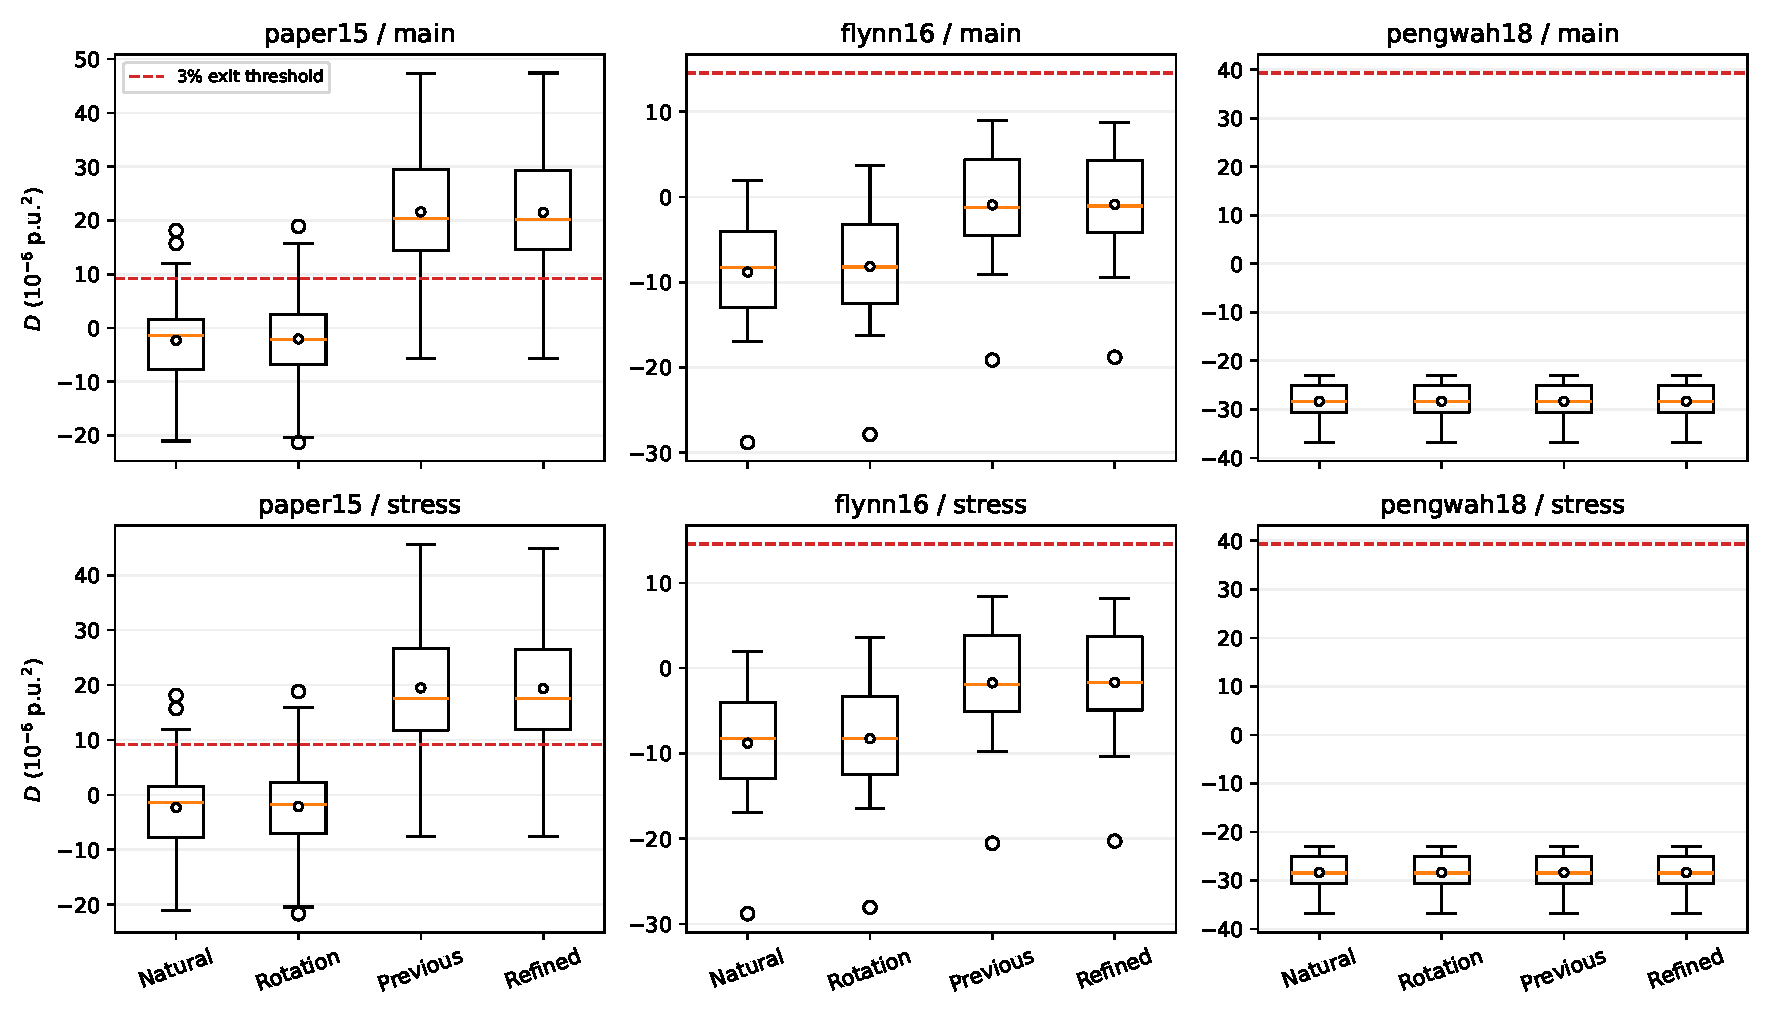
\includegraphics[width=\textwidth]{figures/loss_thresholds.pdf}\caption{冻结报价在独立AC路径上的实际损失差与原3\%排除阈值。箱线为24日结果；圆点表示均值，红线为历史阈值。显示指标是否足以触发选模，不能单独代表真实恢复。}\end{figure}\FloatBarrier

paper15主响应新价/旧价/轮换的实际绝对调节分别为158.61/95.80/201.14 kWh/日；新价平均净调节0.19 kWh/日。新价$D$均值21.505、最小-5.723，阈值9.179（微标幺平方）。

flynn16主响应新价/旧价/轮换的实际绝对调节分别为142.92/116.92/186.02 kWh/日；新价平均净调节-0.92 kWh/日。新价$D$均值-0.867、最小-18.791，阈值14.543（微标幺平方）。

pengwah18主响应新价/旧价/轮换的实际绝对调节分别为0.00/0.00/0.00 kWh/日；新价平均净调节0.00 kWh/日。新价$D$均值-28.351、最小-36.858，阈值39.314（微标幺平方）。

结果需按代价与可行性共同判断：若新价未达95\%、费用增加而实际恢复相同，就不将其作为已验证优于旧价的方法。保留旧价作为对照，下一步应针对参考预测与局部搜索瓶颈收口分析，不能用提高资源或降低选择阈值补出成功。
\subsection{本轮改进的判定}

paper15的新报价相对同费轮换，主响应18条改善、6条相同、0条变差；失配响应17条改善、7条相同、0条变差。新价的实际调节总量低于轮换，因此收益不能仅用“调节更多”解释。原始候选和冻结收缩输出在全部576条记录中错漏一致，改善保留到最终输出。

但相对旧报价，新价主响应仅1条改善、23条相同，失配响应24条全同，日费增加约65.24\%。独立工作概率仅由92.289\%增至93.359\%。flynn的工作概率由34.164\%增至36.123\%，实际仍未恢复。因而本轮没有支持将更贵新价作为默认替代方案，也没有解决95\%规划可行化。

纸面上的尾部初值并非本批收益的唯一解释：paper15最终最好点来自旧价启动的原概率搜索；flynn来自另一启动，但没有实际纠错增益。外层样本数和迭代量也同时改变，因此未作独立消融前，不将增益归因于尾部初始化。

下一步应保留较便宜旧价作为已验证对照，优先核查预测参考残差在新日AC下的失配来源，以及当前资源下阈值是否可达。三个训练日秩至多2的工作分布是具体缺口；继续增加局部迭代不能替代这一核查。本报告保留全部不达标和零收益情况，不以改变3\%、噪声或库存获得正结果。


\section{代码对应、复现及结论范围}
\begin{longtable}{p{.43\textwidth}p{.49\textwidth}}
\toprule 相对研究目录的文件&作用\\\midrule\endhead
\path{dr_heterogeneous_resources/}\newline\path{library.json}&资源、价格、行为及已记录但未启用的预测模板。\\
\path{dr_heterogeneous_pilot/}\newline\path{devices.py}&功率、终端能量、储能SOC控制；名义与随机执行；控制器反向导数。\\
\path{dr_heterogeneous_pilot/}\newline\path{planner.py}&候选残差、原条件概率及完整链式梯度。\\
\path{dr_conditional_gaussian/}\newline\path{conditional_integral.py}&严格有符号L1事件的区间积分、根与梯度诊断。\\
\path{dr_probability_refinement/}\newline\path{tail.py}&精确条件短缺期望及尾部初值。\\
\path{dr_probability_refinement/}\newline\path{refine.py}&预锁协议、可行化/费用搜索、独立核验、调用原AC与冻结评分。\\
\path{dr_newday_weighted/}\newline\path{weighted_selection.py}&复用实际新日加权3\%规则；不调用其默认2\%结果。\\
\path{dr_probability_refinement/}\newline\path{audit.py}&独立重算选择、错漏、设备状态与完整分母。\\\bottomrule
\end{longtable}

每次运行先保存协议、输入与源码SHA-256、环境及种子。价格冻结后才生成新AC路径。断点按记录保存，失败不覆盖，完成记录不重复计算。原始家庭或聚合P/Q/V、完整R/X、报价及设备轨迹留私有目录；公开仅源码、声明配置、汇总、图和本文。

当前能够支持的结论是：在声明资源和预测模型下构造可计算的概率价格问题，并检查报价对固定历史候选的验证和最终输出是否产生改善。其价值不能由概率梯度、方差、调节量或训练拟合单独代替。此价格优化形式也能用于其他来源的候选；本批WZZT的具体作用是与RNJ共同提供历史结构和联合参数，尚未证明这种概率优化形式为WZZT所独有。

仍需后续改进的主要部分是背景与参考误差的预测校准、实际行为及费用来源、候选池代表性；这三项与数值求解是否更充分是不同问题。扩大网络之前，应先确认目标事件在原规则下有效、代价合理，且独立实际路径能保留改善。

\begin{thebibliography}{9}
\bibitem{rockafellar} R. T. Rockafellar and S. Uryasev.
Optimization of Conditional Value-at-Risk. \emph{Journal of Risk}, 2(3):21--41, 2000.
开放作者稿（1999-09-05），本次核对方法定义及定理1，印刷页3--5：
\url{https://sites.math.washington.edu/~rtr/papers/rtr179-CVaR1.pdf}。
\end{thebibliography}
\end{document}
